\documentclass[12pt,a4paper]{article}
\usepackage[portuguese]{babel}
\usepackage[a4paper]{geometry}
\usepackage[utf8]{inputenc}
\usepackage{lmodern}      % letra, símbolos, etc.
\usepackage{cmap}
\usepackage{setspace} % Espaçamento entre linhas 
\usepackage{microtype} % espaçamento entre letras e palavras, colocar depois da fonte
\usepackage{siunitx} % unidade si 
\sisetup{output-decimal-marker = {,}}
\usepackage[version=4]{mhchem}
\usepackage{caption} % caption
\usepackage{subcaption} % caption   
\usepackage{graphicx}     % gráficos
\usepackage{tabularx}     % tabelas
\usepackage{booktabs}  
\usepackage[table]{xcolor} % cores
\usepackage{multirow}
\usepackage{makeidx}
\usepackage{ragged2e}
\addto\captionsportuguese{\renewcommand{\refname}{Referências}}
\usepackage[colorlinks=true,citecolor=black,linkcolor=black,bookmarks=true]{hyperref}
\usepackage{natbib}
\usepackage{float}
\usepackage{indentfirst}

\onehalfspacing

\begin{document}

\pagenumbering{arabic}

\thispagestyle{empty}
\begin{minipage}{\textwidth}\centering
Universidade de São Paulo \\
Instituto de Ciências Matemáticas e Computação \\
Desenvolvimento de Código Otimizado - SSC 0951 \\
\end{minipage}

\vspace{5cm}

\begin{minipage}{\textwidth}\centering
\Large Relatório Trabalho 2  \\
\vspace{2cm}
\Large \textbf{Ferramenta de \textit{Profiling} - \textit{gproof}}
\end{minipage}

\vspace{3cm}

\begin{minipage}{\linewidth}\centering
\begin{enumerate}
     \item Lucas G. Meneses   \space \space \space \space \space \space  Número: 13671615
      \item Henrique S. Marques  \space \space Número: 11815722
      \item Carlos F. C. Lemos  \space \space \space \space Número: 12542630
      \item Eduardo S. Rocha  \space \space \space \space \space \space Número: 11218692
\end{enumerate}
\end{minipage}

\vfill

\begin{minipage}{\linewidth}
\centering\today, \\
São Carlos, SP, \\
Brasil
\end{minipage}

\clearpage
\thispagestyle{empty}

\tableofcontents

\section{Introdução}

A importância do \textit{profiling} de códigos é inegável no cenário de desenvolvimento de software. Trata-se de uma prática crucial que permite aos programadores identificar gargalos de desempenho e aprimorar a eficiência de suas aplicações. Com a complexidade cada vez maior dos sistemas de \textit{software} atuais, compreender detalhadamente o tempo de execução de diferentes funções e a alocação de recursos se tornou uma etapa essencial para garantir a entrega de produtos de alta qualidade e desempenho robusto.

Como exemplo, imagine um aplicativo de comércio eletrônico que está sofrendo com lentidão e baixo desempenho. Sem a prática do \textit{profiling} de código, os desenvolvedores podem ficar às cegas na tentativa de resolver o problema. No entanto, ao realizar o \textit{profiling}, eles podem identificar que uma função de pesquisa está consumindo uma quantidade desproporcional de recursos de CPU e que a alocação de memória está fora de controle durante as consultas. Com essa análise precisa, os desenvolvedores podem otimizar essa função crítica, reduzindo o tempo de resposta e garantindo que o aplicativo funcione de maneira eficiente, proporcionando uma melhor experiência ao cliente e evitando a perda de vendas devido à lentidão. 

Nesse contexto, uma ferramenta conhecida no ambiente de desenvolvimento é o \textit{gproof}, uma ferramenta de \textit{profiling} de código aberto que oferece uma variedade de recursos poderosos para a análise de desempenho de \textit{software}. Por meio do rastreamento do tempo de execução de funções, identificação de chamadas recursivas e análise abrangente de alocação de memória, o \textit{gproof} permite que os desenvolvedores compreendam a fundo o desempenho de seus códigos. Além disso, com a geração de relatórios detalhados e visualizações gráficas intuitivas, o \textit{gproof} capacita os desenvolvedores a tomar decisões embasadas em dados concretos, priorizando esforços de otimização e melhorando o desempenho geral das aplicações.

\section{Metodologia} \label{sec:metodologia}

Para a realização de todos os experimentos, foi utilizado um computador rodando o Sistema Operacional Ubuntu, cuja CPU é um Intel Core i5 6600k com frequência de \textit{clock} de \SI{3,5}{\giga\hertz}, 4 núcleos e 4 \textit{threads}. Quanto à memória, o computador faz uso de \SI{16}{\giga\byte} de RAM do tipo DDR4, cache L1 de dados e de instruções ambas 8-\textit{way} com $4 \times \SI{32}{\kilo\byte}$ de capacidade, L2 4-\textit{way} $4 \times \SI{256}{\kilo\byte}$ e L3 12-\textit{way} de \SI{6}{\mega\byte}.

Nesse sentido, o perfilador \textit{gproof} foi utilizado 10 vezes para avaliação dos tempos de execução de 3 algoritmos de ordenação com comportamento assintótico $O(n^2)$:
\begin{itemize}
    \item \textit{Bubble Sort}
    \item \textit{Selection Sort}
    \item \textit{Insertion Sort}
\end{itemize}

Assim, em cada execução, o mesmo vetor aleatório com $100000$ inteiros de 8 $bytes$ foi ordenado por cada um dos 3 algoritmos citados acima, de modo que, entre uma ordenação e outra, a memória cache tenha sido limpa, evitando que haja interferências na quantidade de cache \textit{misses}, tornando, pois, a comparação entre os algoritmos mais justa. Ademais, as médias aritméticas e intervalos de confiança (\SI{95}{\percent}) referentes às 10 execuções foram calculados, com intuito de melhor avaliar os resultados obtidos. Por fim, o código, os dados brutos e as figuras geradas estão disponíveis em repositório aberto via \href{https://github.com/greffao/Optimizing-Code}{GitHub}.  

\section{Resultados}

Com objetivo de melhorar a visualização dos resultados obtidos com a utilização do perfilador \textit{gproof}, \textit{plotamos} os grafos das chamadas de funções. Conforme será discutido posteriormente, os tempos de execução foram bastante consistentes ao longo do 10 execuções, apresentando poucas variações. Dessa forma, apesar de não representar com total fidelidade o resultado final do experimento, a Figura \ref{fig:grafo}, referente ao grafo da primeira execução, indica o comportamento padrão dos algoritmos avaliados neste estudo.\protect\footnotemark

\footnotetext{Como já citado na Seção \ref{sec:metodologia}, todos os 10 grafos podem ser encontrados no repositório do \href{https://github.com/greffao/Optimizing-Code}{GitHub}, acessando $Atividade2\rightarrow Resultados2\rightarrow Grafos$.}

\begin{figure}[H]
\centering
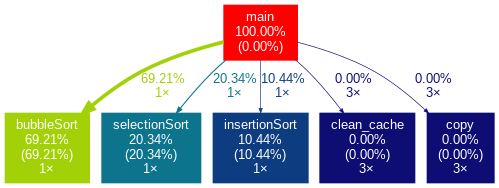
\includegraphics[width=0.90\linewidth]{Figures/grafo.png}
\caption{Grafo das chamadas de funções para o primeiro experimento realizado com os algoritmos \textit{Bubble Sort}, \textit{Selection Sort} e \textit{Insertion Sort}. As funções auxiliares \textit{clean\_cache} e \textit{copy} foram utilizadas para \textit{reset} da memória cache e cópia dos dados entre vetores (algoritmos \textit{in place}), respectivamente.}
\label{fig:grafo}
\end{figure}

Como pode ser visto no grafo, o algoritmo \textit{Bubble Sort} foi o mais custoso em termos de tempo de execução, consumindo, aproximadamente, \SI{70}{\percent}, do tempo total gasto para finalizar o programa, seguido do \textit{Selection Sort}, com \SI{20}{\percent}, e do \textit{Insertion Sort}, com \SI{10}{\percent}. 

Nesse sentido, o comportamento observado é totalmente condizente com o esperado ao se avaliar as características particulares de cada heurística: o \textit{Bubble Sort} é um algoritmo de ordenação ineficiente, pois exige muitas trocas e comparações. Isso o torna consideravelmente mais lento do que o \textit{Selection Sort} e o \textit{Insertion Sort}, os quais, apesar de possuir o mesmo comportamento assintótico quadrático, envolvem menos operações de comparação e troca, na maioria dos cenários (\textit{e.g} vetor aleatório). De maneira mais quantitativa, os resultados obtidos também puderam ser analisados através das médias aritméticas e dos intervalos de confiança (\SI{95}{\percent}). Os valores encontrados podem ser visualizados com a Tabela \ref{tab:media_confianca} e com a Figura \ref{fig:media_confianca}.

\begin{table}[H]
\centering
\caption{Médias aritméticas e intervalos de confiança (limites inferior e superior, \SI{95}{\percent}) das 10 execuções de cada um dos três algoritmos quadráticos avaliados neste estudo.}
\label{tab:media_confianca}
\begin{tabular}{lSSS} \toprule
{Algoritmos} & {Média} & {Limite Inferior} & {Limite Superior} \\ 
& {(\si{\second})} & {(\si{\second})} & {(\si{\second})}  \\ \midrule
{\textit{Bubble Sort}}     & {38,559} & {37,803} & {39,315}  \\
{\textit{Selection Sort}}  & {11,206} & {10,951} & {11,461}  \\
{\textit{Insertion Sort}}  & {6,290}  & {6,142}  & {6,438}  \\ \bottomrule
\end{tabular}
\end{table}

\begin{figure}[H]
\centering
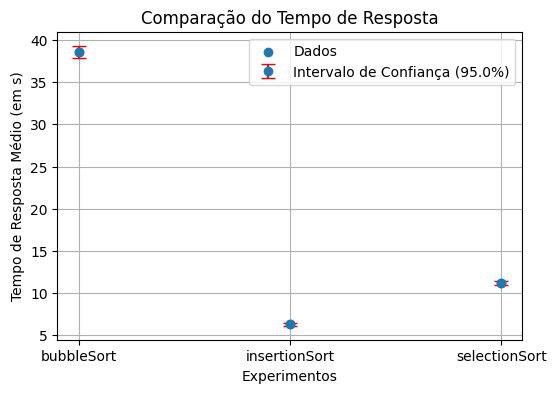
\includegraphics[width=0.90\linewidth]{Figures/media_confianca.jpg}
\caption{Tempos de resposta (\si{\second}) em função do experimento realizado. Os círculos azuis indicam a média dos dados obtidos para cada experimento e as barras vermelhas mostram o intervalo de confiança de \SI{95}{\percent}.}
\label{fig:media_confianca}
\end{figure}

\section{Conclusões}

A importância do \textit{profiling} de códigos é fundamental no desenvolvimento de software, permitindo aos programadores identificar gargalos de desempenho e aprimorar a eficiência das aplicações. Nesse contexto, a ferramenta de \textit{profiling} de código aberto \textit{gproof}, testada neste trabalho, se destaca, oferecendo recursos avançados para a análise de desempenho, incluindo o rastreamento de tempo de execução de funções, com relatórios e visualizações gráficas para embasar decisões de otimização. 

Os resultados demonstram o uso efetivo do perfilador \textit{gproof} para visualizar o comportamento de algoritmos de ordenação quadráticos, especificamente o \textit{Bubble Sort}, \textit{Selection Sort} e \textit{Insertion Sort}. Notavelmente, o \textit{Bubble Sort} consumiu cerca de \SI{70}{\percent} do tempo total de execução, seguido pelo \textit{Selection Sort} com \SI{20}{\percent} e o \textit{Insertion Sort} com \SI{10}{\percent}. Esses resultados estão alinhados com as expectativas, visto que o \textit{Bubble Sort} é conhecido por ser um algoritmo ineficiente devido às trocas e comparações excessivas, enquanto o \textit{Selection Sort} e o \textit{Insertion Sort} são mais eficientes em média. A análise quantitativa com médias e intervalos de confiança reforça as conclusões, destacando a disparidade nos tempos de execução entre os algoritmos.


\end{document}